\documentclass[12pt]{article}

\setlength{\parskip}{1em}

\usepackage[T1]{fontenc}
\usepackage[english]{babel}
\usepackage{textcomp}
\usepackage{amsfonts}
\usepackage{graphicx}
\usepackage{hyperref}
\hypersetup{
  colorlinks=true,
  linkcolor=blue,
  urlcolor=blue,
  pdftitle={IFE Project: final report}
}

\title{IFE Project: Final report}
\author{Adrien Burgun, Jules Ramos}
\date{Spring 2020}

\graphicspath{{report/}}

\begin{document}

\maketitle

\begin{abstract}

This semester's project for the \textbf{IFE} (Algorithmics and Programming) class was a game of Belote, programmed in \textbf{C}.
It had to:

\begin{itemize}
\item have a main menu, featuring a leaderboard, a quit button and a play button
\item have a pseudo artificial intelligence against which the player would play
\item let the user and make the artificial intelligence bid at the beginning of a game
\item let the user and make the artificial intelligence play card during the game
\item show the cards of the user during the game
\item show the cards of the current fold
\item save the number of wins of a player in a leaderboards file
\item distribute cards to the different players
\item check that the player plays according to the rules
\item calculate scores
\item define who wins the round after 4 cards are played
\item count the total amout of points and check who fulfilled their contract
\end{itemize}

This document is a report of our project, the making of it and the end result.

\end{abstract}

\newpage
\tableofcontents
\newpage

\section{Project structure}

We decided to use \href{https://git-scm.com/}{Git} for the entirety of the project.
\textbf{Git} is a Version Control System, which let us work on two separate \textit{branches} at the same time, which we later merged together, as to not interfere with each other.
It has also proven itself to be very useful to find the origin of bugs (see \hyperref[issues]{Issues}).

The code is hosted on \textbf{GitHub} and is available here:

\url{https://github.com/adri326/ife-project}

An \textit{aftermath} branch has been created to host fixes to the \hyperref[issues]{issues} that we found in the game after it was handed out.

To support each of our usual working environment, we created a \textbf{CMake} configuration script and two \textbf{Code::Blocks} projects (one for the game itself and one for the tests).
Instructions on how to compile using either tool can be found on the repository's \textit{README.md} file.
One will either need a terminal, \textbf{CMake} and the \textbf{SDL2} libraries installed on their system or \textbf{Code::Blocks} on Microsoft Windows (preferably using the MinGW suite).

The code was formatted using \textbf{clang-format}, which is a tool part of \textbf{LLVM}'s suite.
It, however, did not give us the flexibility that we hoped it would.

\subsection{Directory structure}

\begin{description}
\item[/] - the root directory, it contains this report, project files, config files and the license.
\item[/src] - all of the source files of the game: \textit{src/ai.c} contains the artificial intelligence-related code, \textit{src/display.c} the graphical code, \textit{src/game.c} the game's logic code, \textit{src/leaderboards.c} the leaderboards' code and \textit{src/rules.c} the rules of the game.
\item[/lib] - the required libraries to build on Microsoft Windows.
\item[/resources] - the graphical resources for the game (textures, the charset).
\item[/cmake] - a \textbf{Git} dependency, containing \textbf{CMake} scripts to locate the game's required libraries on various platforms.
\item[/report] - contains the pictures used in this report.
\end{description}

\section{Our creation process}

\subsection{The different structures}

Before coding anything for the game, we first had to create the structures to hold all of the data of a game. This includes the status of the different cards and players.
We started by defining the simplest structure elements - cards, to then scale up. This is mainly because each structure contains elements of lower structures.

After discussing it, we decided that the best way to handle the cards would be to create a structure which would contain their two characteristics: their number (or value) and their color (or type).
Rather than representing colors with numbers, which would easily be confusing for anyone reading the code, we created an enumeration type (\textit{CardColor}) with the 4 colors (\textit{HEARTS}, \textit{TILES}, \textit{CLOVERS}, \textit{SPIKES}) and a \textit{VOIDCARD} for ``empty'' card slots.
For the number, using integers seemed more natural so we kept it that way after defining our own convention.

Because card numbers can be fully contained within an 8-bit unsigned integer, we decided to store them using such a type (\textit{uint8\_t}).

The player structure required more information: it had to store its own hand (\textit{Card cards[8]}) and various scores (declaration points, belote points, tricks won and the total number of points won).
Storing these scores in the game structure would have required 4 variables per kind of data in the general game structure, which we felt was a bad idea.

The game structure contains 4 instances of the player structure.
It also stores various informations about the active contract; we created two enumeration types (\textit{ContractType} and \textit{TrumpColor}) to represent which kind of contract was agreed upon or is being contested and a trump color.
We ended up storing the contract kind (\textit{active\_contract}), its bid value (\textit{contract\_points}), the trump color with which it was bid (\textit{active\_trump}) and who bid it (\textit{general\_attacker}).
\textit{ContractType} also has two values for coinche and surcoinche, rather than having another separate value for it. Special contract kinds ("capot" and "general") which were coinched are differentiated through the contract value.

The current fold is stored as a 4-card list, \textit{pli}, the color it was initiated with in \textit{trick\_color} (to check if a move is valid) and lastly whether or not it was cut (using a trump card) in \textit{trick\_cut}.

\subsection{Coding the rules of the game}

For this part of the game, we actually decided to code from the end of an 8-trick turn to its beginning. That way we avoided forgetting to introduce variables that would be needed later.

Therefore, we began by creating the function that computes the points of each team at the end of the turn.
This function was not the most complex in itself but having to create all the structures, enumerations and variables that would be required made it harder.
According to the rules, we had 4 cases to deal with: we compute the points of the winning team that actually took the contract, the loosing team in the same scenario, the winning team that is not the team which took the contract and the loosing team that took the contract.
This was translated as 2 if-else structures inside a general if-else structure.
We check if the team we are computing the points for is the winning team, and then if it is the contracted team.
For each scenario, we then compute the points by following the rules with a switch letting us check if the contract was a coinche or surcoinche as those have a multiplier to apply.
The different variables created are used here to compute these points: we call the total trick points of each player of the concerned team, the contract type, the belote points, …

For the player structures, we decided to use pointers rather than creating another copy of them to optimize the game.
In the pointer declaration, we inserted an if-else like structure in order to determine which players are concerned and which players lost for the specific case of the contracted team winning.
When we first wrote the function, we used to switch to do so but when we tried to optimize it this solution appeared as lighter for the code and more efficient.

\subsection{Checking contracts}

To easily manipulate the player structures, we used pointers and as the 4 players had to change depending on what team was contracted and had to be checked we used a switch to give each player their role, attacker or defender.
The function had to return the name of the winning team, defenders if the contract was not achieved and attackers otherwise (using an easy enumeration to name the two teams).

To do so, we initially created 2 functions using a switch to return the name of the wanted team, defending or attacking.
These functions returned a \textit{Teams} enumeration variable that was then returned by the main contract checking function.
When we optimized this part of the code, we determined that using a define would be easier and better.

As the \textit{Teams} enumeration only has 2 elements, we could define the attackers winning as a straightforward return of the enumeration element held by the contracted team variable and the defenders winning as the opposite element.
Then we had the easiest case to code: the contracted team had less total trick points than 82 and instantly lost, the function returns the name of the defenders.
After that came the case where the contracted team had more than 82 trick points.
We then had to check every contract possible that’s why we used a switch on the contract type.
The easiest case is a "classic" contract where the attacking team needs to reach a particular number of points by just adding different point variables linked to both players.
Then came the capot: the two attacking players needed to have won all of the tricks hence the number of tricks won by each player variable.
We just had to check that they won 8 tricks together.
The general had the same logic but with only one player whose position was stocked in the \textit{general\_attacker} variable.
Finally came the coinche and surcoinche which have the exact same logic but with the winning team being opposite.
For each one, we had to use the contract points variable to check what type of contract was contested and then we needed to check if the right team, the defending team for a coinche and the attacking one for a surcoinche, achieved the contract.
Each contract check was then the same as previously stated.
A switch was again used to describe the different possibilities.
Finally, a security return that should never be reached was added because we did not add a default case (that could have been the chosen color contract) to the main switch therefore there is for the compiler a possibility that nothing would be returned even though in real life this would not be possible as a contract type would always be chosen.

Then, still going backwards in a turn, we had to code the trick points. This was easy: we just have to sum the values of the 4 cards played and add 10 points if it was the 8th trick. The value of the cards is determined in another function that we can use again in many different cases. It is again a very logic function: a switch case to determine which trump is active then for the all trumps and no trump a switch to give each card a point value depending on the card value (7, Jack, Ace,…). In the case of a chosen color trump, the same thing is done with an additional step: we must check if the card color is the same as the trump or not. As we had to separate the card color from the trump color, we use a property of enumerations: each element is represented by an integer beginning at 0. We placed the card colors and the trump colors in the same order therefore we can just check if these two integers are the same and give the right point value to the card.

The following function checks if a move is possible or not, returning 0 if not, 1 if it is and 2 if it is but cuts the trick. This function is complex on a logic level but in the code is only several if-else structures and switches one after another. Detail was\_anything\_played here. To create this function, we first drew a diagram of the different branches of possibilities. We won’t detail it here as it is literally a logic translation of the rules of the game. In this function we have to check the hand of the player several times that’s why we use for statements to check the cards one by one. We are either looking for the trick or trump color. We set a Boolean variable as true and if a card with the searched color is found we change it as false. That way we know that if the variable remains true then the player does not have the color in their hand. For the specific case of a player not wanting to cut a trick but not having the trick color in their hand even though they have a trump card, we have to check if the player’s partner is leading the trick hence the trick leader variable.

That trick leader can be used as the trick winner at the end of the trick and has to be determined by a last function in the rules. This function will be call after the move check. This is a very logic function again mostly using if-else structures. First with pointers we get the 4 cards of the trick, empty of not, and the current leading card. Then we check if the move checked is the first of the trick by checking if the type of the 3 other cards is VOIDCARD or not. If it is, we can initialize the player as leader and check if they played a trump or not with the same integer logic as previously. If they do, then the trick is already stated as cut. For an all-trump and no-trump case, this won’t be impactful. If it is not the first move, then we can check if the trick was cut or not. If it was, we check if the player played a trump or not and if the leader played a trump or not. If both did, then we compare the values of the cards to determine the new leader. If the leader did not play a trump but the player did, then the trick is cut (the cut variable got changed before this function was called and after the move check function returned 2) and the player gets the lead. If the player does not play a trump and the leader did, then the leader remains the same. If the trick was not cut, then we don’t need to worry about trumps. This is also the case that will be used for an all trumps and no trump. The logic is similar to the previous case: we check if the player played a card of the trick color. If they did not, then they can not win against the leader. If they did, we have to check the value of the cards. A safety return was again added for the same reason as last time. Each time we compare card values, we must remember that 7, 8 and 9 for a non-trump card have a value of 0 so we also have to check the card value of the card structure to determine which one is better.

\subsection{Declarations}

The game of Belote lets players declare special sets of cards that they have in hand in order to earn points, at the cost of revealing part of their cards to the other players.

In order to efficiently check declarations, we needed a function that would be able to take the cards the player proposed and returned the value of them together. There are two main kinds of declarations: 4 times the same card with different colors and following value cards. Therefore, our function is separated in two thanks to an if-else statement. If all the given cards have the same value, knowing that the cards would always be ordered before being given to this function and that "empty" slots would have a value of 0, we just have to realize a switch on the value of these 4 first cards of the given array to get the declaration value. In the case that they do not have the same value. We assume the player wants to declare following value cards. In order to check what relevant cards are proposed, we use 5 Boolean variables representing the presence of these cards and we check every card of the array given one by one. Depending on what cards are here, we then return the proper value.
Because of a lack of time, we did not add an anti-cheat test to see if the following cards are from the same color which would have been done by adding a for statement checking following cards color by color.

The cards that have been revealed are stored in an 8-bit mask, each bit representing if the corresponding card of the player's hand has been revealed.

This feature ended up not being used, as we did not have enough time to implement a graphical interface for the player to use it, nor did the artificial intelligence include it.
The \textit{play\_card} function, which is used by the player and the AI to play a card, did not include a way to shift the revealed card mask.

\subsection{The dealing phase}

For the function managing the dealing phase, the biggest issue was to always check if an AI or the human player has to play as they have separated functions to do so.
That’s why each time a contract has to be proposed or passed we have to check with an if-else statement who is playing.
Every dealing phase has to begin with the 4 players announcing or passing, therefore we do so 4 times.
If after these 4 times the contract value is still 0, it means nobody announced a contract and therefore we have to redistribute cards.
In the first version of this function, the variable \textit{previous\_contract\_points} took its value after the first player announced.
That way, if the value of the contract is different from 0 and equal to this first value, we know 3 players passed and the contract was taken, symbolized by a return value of 1.
If not, a for loop was established for each player to deal one after another, with a variable counting consecutive passes until it came back to the last player to announce.
This first version had a default: it did not count the number of passes in the initial loop.

\label{previous-contract-points}

In a subsequent modification of this function, the \textit{previous\_contract\_points} was put after the initial loop, rendering it useless.
This means that it only allowed one turn of bidding - the AI couldn't overbid or coinche what the player played.
The origin of this issue could be found using \textbf{Git}, by looking at the history of the \textit{src/game.c} file.

The current implementation of the artificial intelligence did not have any case where it could overbid or coinche/surcoinche the player's bid, so this bug went unnoticed.

\subsection{The graphical interface}

The graphical interface was made using \href{https://www.libsdl.org/index.php}{Simple DirectMedia Layer 2} and its associated libraries (\textbf{SDL2\_image}, \textbf{SDL2\_mixer} and \textbf{SDL2\_ttf}).
We ended up only needing \textbf{SDL2} and \textbf{SDL2\_image}.

The different assets are first loaded using \textbf{SDL2\_image}.
They are then upscaled using our \textit{zoom\_surface} function - which is inspired by \textbf{SDL2\_gfx}'s \textit{\_zoomSurfaceRGBA} function - and converted into instances of \textit{SDL\_Texture}.
Whenever these assets are needed, they are copied onto the window.
Before the game exists, we clear these textures from the memory.

Most of the textures are pixel art. We tried making them as small as possible:
each glyph (character) is 5 pixels wide and 5 pixels high, the cards are 19 by 28 pixels big.
It would have been both tedious and unmaintainable to manually texture all of the 32 cards.
The different elements making up a card have thus been separated into several textures and are assembled during load time.

Glyphs are arranged in an 8x8 grid (\ref{charset}).
Upon loading, they are split into individual textures and colored to achieve the different colors that we use in the game.
Outside of the title and the cards themselves, all of the graphics have been done using characters.

\begin{figure}[ht]
  \caption{\label{charset} The charset; the character `M' is highlighted}
  \begin{center}
    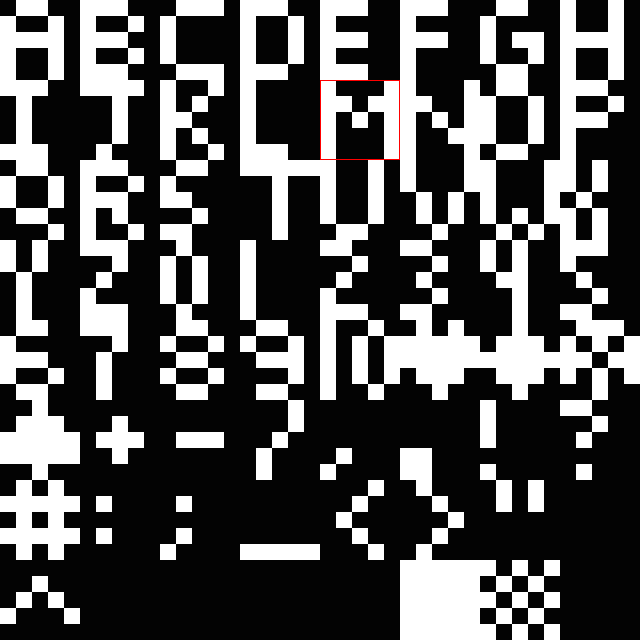
\includegraphics[width=0.75\textwidth]{charset}
  \end{center}
\end{figure}

Due to the unwieldiness of the \textit{C} language, we did not create a central graphics loop.
Instead, these have been reduced to a small form and are present in the different parts of the code that need them:
For instance, a loop runs while the user is asked to play a card. This loop highlights cards that the user can play when they are hovered.
As soon as the user plays one of these cards by clicking on it, the loop stops and soon after, another loop is entered, which displays the animation of that card being played.
This, however, means that we couldn't have many animations. The game sometimes feels a little ``jumpy'' whenever a screen turns into another one without transition or user interaction.

\begin{figure}[ht]
  \caption{Screenshot of the card drafting process}
  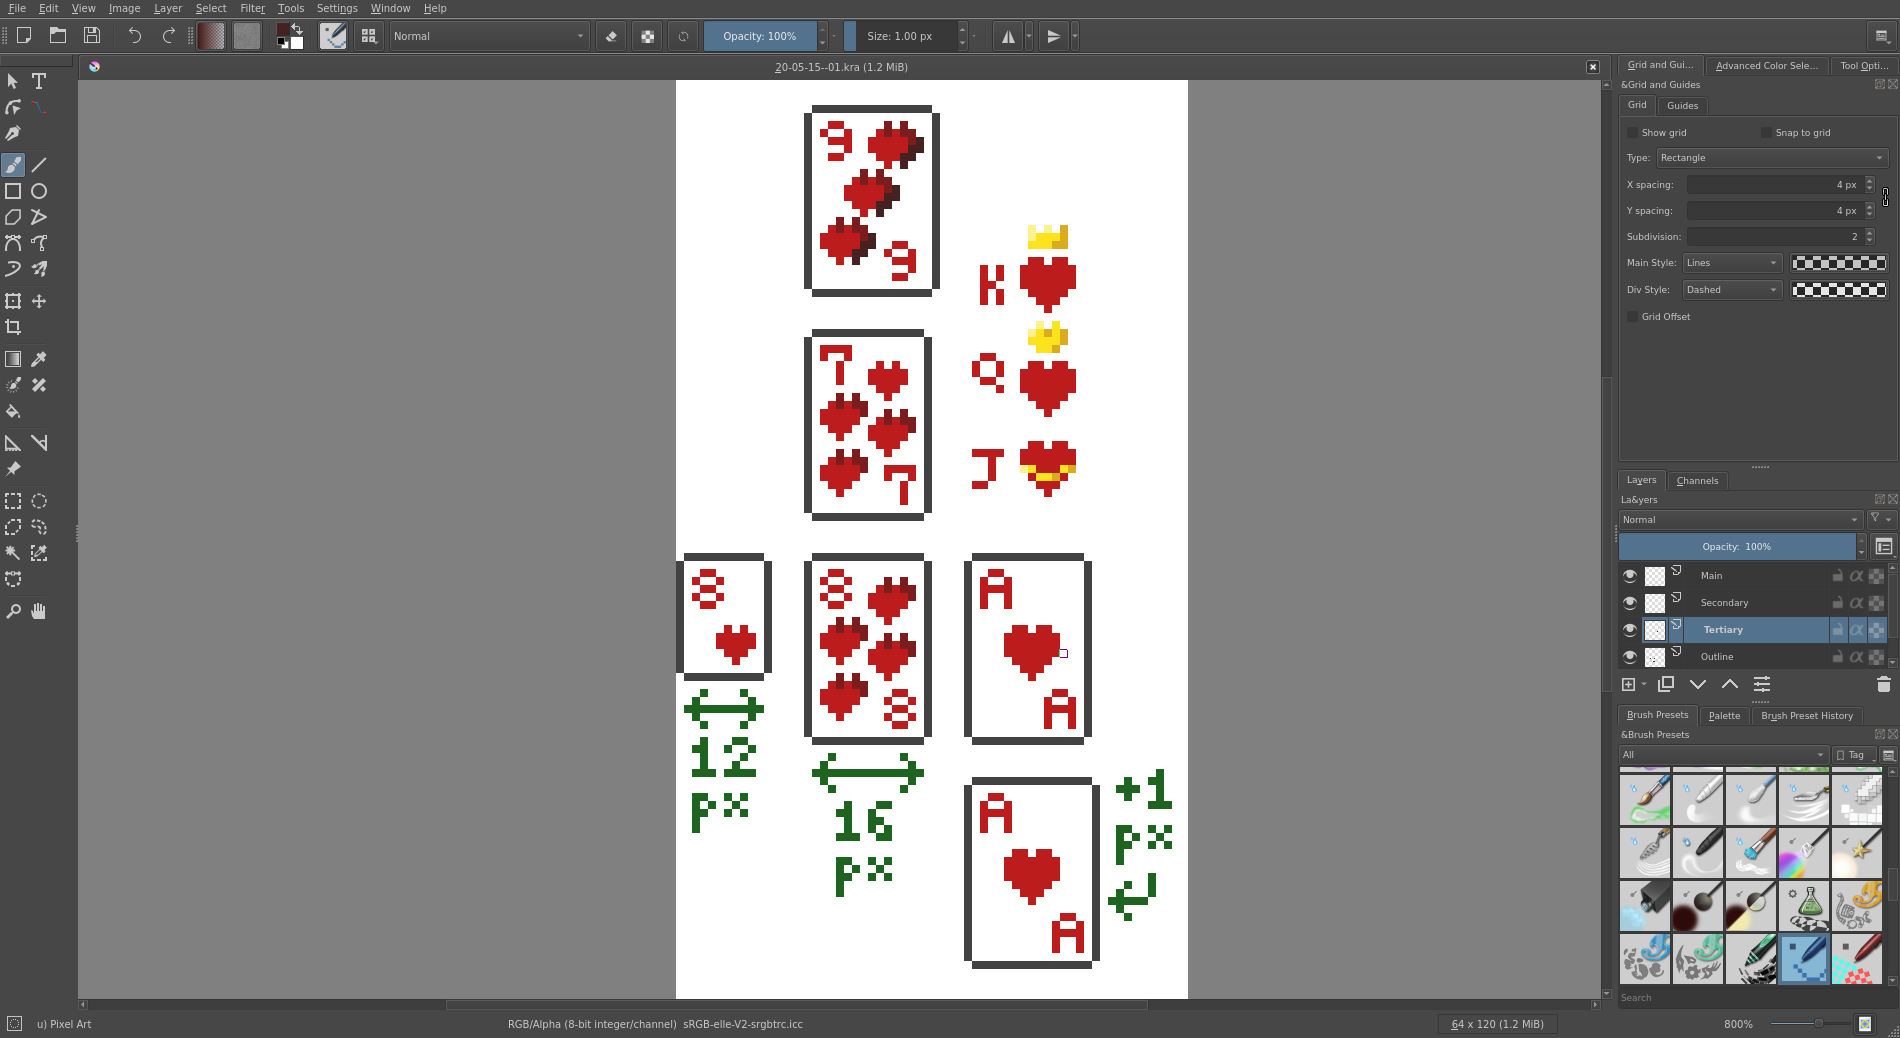
\includegraphics[width=1.0\textwidth]{draft-screenshot}
\end{figure}

\begin{figure}[ht]
  \caption{Screenshot of the game}
  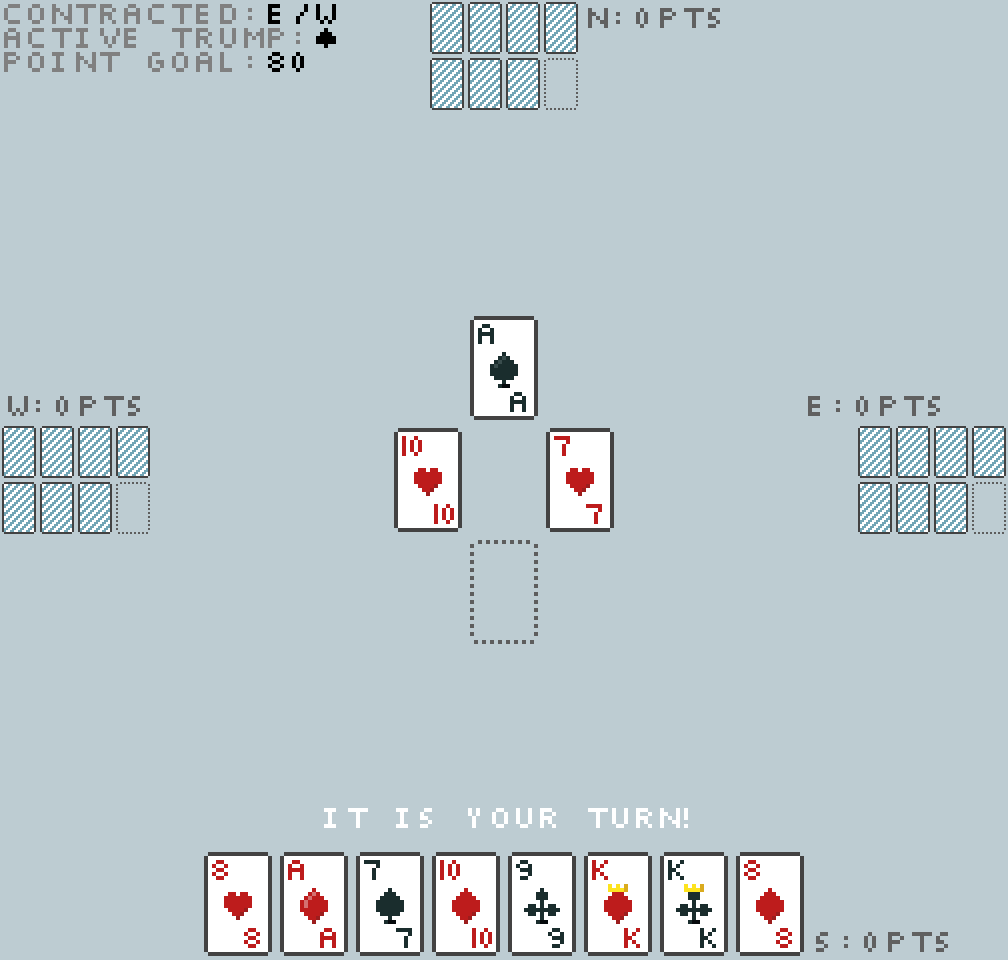
\includegraphics[width=1.0\textwidth]{game-screenshot}
\end{figure}

\subsection{Leaderboards}
\label{leaderboards}

Leaderboards were one of the last features of the game that we implemented.
They are accessible from the main menu and at the end of a won game.

Akin to the pixel art used for the graphics, we implemented leaderboards by having the user enter a 3-letter, case-insensitive name.
It is then stored in a file, \textit{leaderboards.txt}.

The storing process is as follows:

\begin{itemize}
\item The \textit{leaderboards.txt} file is read and the relevant line, if present, is extracted from it (in \textit{get\_score}).
\item The previous total score and win count is summed with the current score and win count of the last game.
\item The \textit{leaderboards.txt} file is read once again. Each line, excluding that of the current player's name, is copied to another, temporary file, \textit{leaderboards.txt$\sim$}. (in \textit{set\_score})
\item The \textit{leaderboards.txt$\sim$} file is read and each line is copied to the \textit{leaderboards.txt} file. (in \textit{append\_score})
\item The new score and win count is appended to the \textit{leaderboards.txt} file. (in \textit{append\_score})
\item The \textit{leaderboards.txt$\sim$} file is deleted (see \hyperref[issues]{Issues})
\end{itemize}

\section{Unit testing}

We decided to have Unit Testing for the different functions that make up the game's logic.
This is to be sure that these work well and to prevent any issue when modifying these functions.

We ended up implementing our own testing tool set (assertions, test output, etc.) using \textit{C} macros and compiler extensions when available.
These can all be seen in the \textit{test/test.h} file.
The tested function had to not have any graphical aspects to them. We thus had to have a compile-time definition set by \textbf{CMake} or \textbf{Code::Blocks} to selectively target out includes and pieces of code handling such graphical aspects.
Compiling the code using the \textit{Makefile} generated by \textbf{CMake} when doing any graphical thing was very useful in these cases, as both targets (the game itself and the tests) are by default compiled.
An error would thus emerge if any code that had to be excluded from the tests was forgotten.

These tests let us catch a few bugs in the code.
For instance, the \textit{turn\_points} function would incorrectly add the declaration points to the total points in one of the test cases. This was caught by one of the tests and was then fixed.

\section{Issues}
\label{issues}

These are the issues that we noticed in the game at its release point:

\begin{itemize}
\item The declaration of \textit{previous\_contract\_points} has been misplaced. \ref{previous-contract-points}
\item Due to its name and because it was later reused when coding the dealing phase, \textit{general\_attacker} is not handled well in the contract checking function.
\item The game's result screen displays the north/south team's score for both teams.
\item The game fails to create a new \textit{leaderboards.txt} file when it is non-present. \ref{leaderboards}
\item The temporary \textit{leaderboards.txt$\sim$} is not deleted. \ref{leaderboards}
\end{itemize}

\end{document}
